\section{V-Modell}

\subsection{Kurzbeschreibung}
\subsubsection{V-Modell 97}
Das V-Modell in seiner ursprünglichen Form wird auch \textbf{V-Modell nach Boehm} genannt, es wurde 1979 erstmals entwickelt und im Jahr 1997 zum \textbf{V-Modell 97} weiterentwickelt. Dieses folgt dem in Abbildung \ref{abbildung_VModell97} dargestellten Pfad.

Das Modell gliedert sich in einen linken und einen rechten Ast, die durch die \textit{Codierungsphase} getrennt werden. Während sich der Projektfortschritt im linken Ast befindet, werden nach und nach verschiedene Spezifikationsdokumente erzeugt, welche im Anschluss an die Codierungsphase, also im rechten Ast eine Bedeutung haben. Der rechte Ast beinhaltet Tests, welche sich jeweils auf das im linken Ast auf der selben Ebene entstandene Spezifikationsdokument beziehen. Die erste Ebene, die im Bild gelb umrandet ist, beschäftigt sich dabei mit der \textit{Validierung}. Diese beantwortet die Frage, ob das richtige Produkt geliefert wurde. Analog beschäftigen sich die verbleibenden Phasen mit der \textit{Verifikation}, also der Prüfung, ob das Produkt den definierten Anforderungen im Bezug auf innere und äußere Qualität folgt.

\begin{figure}[H]
    \centering
    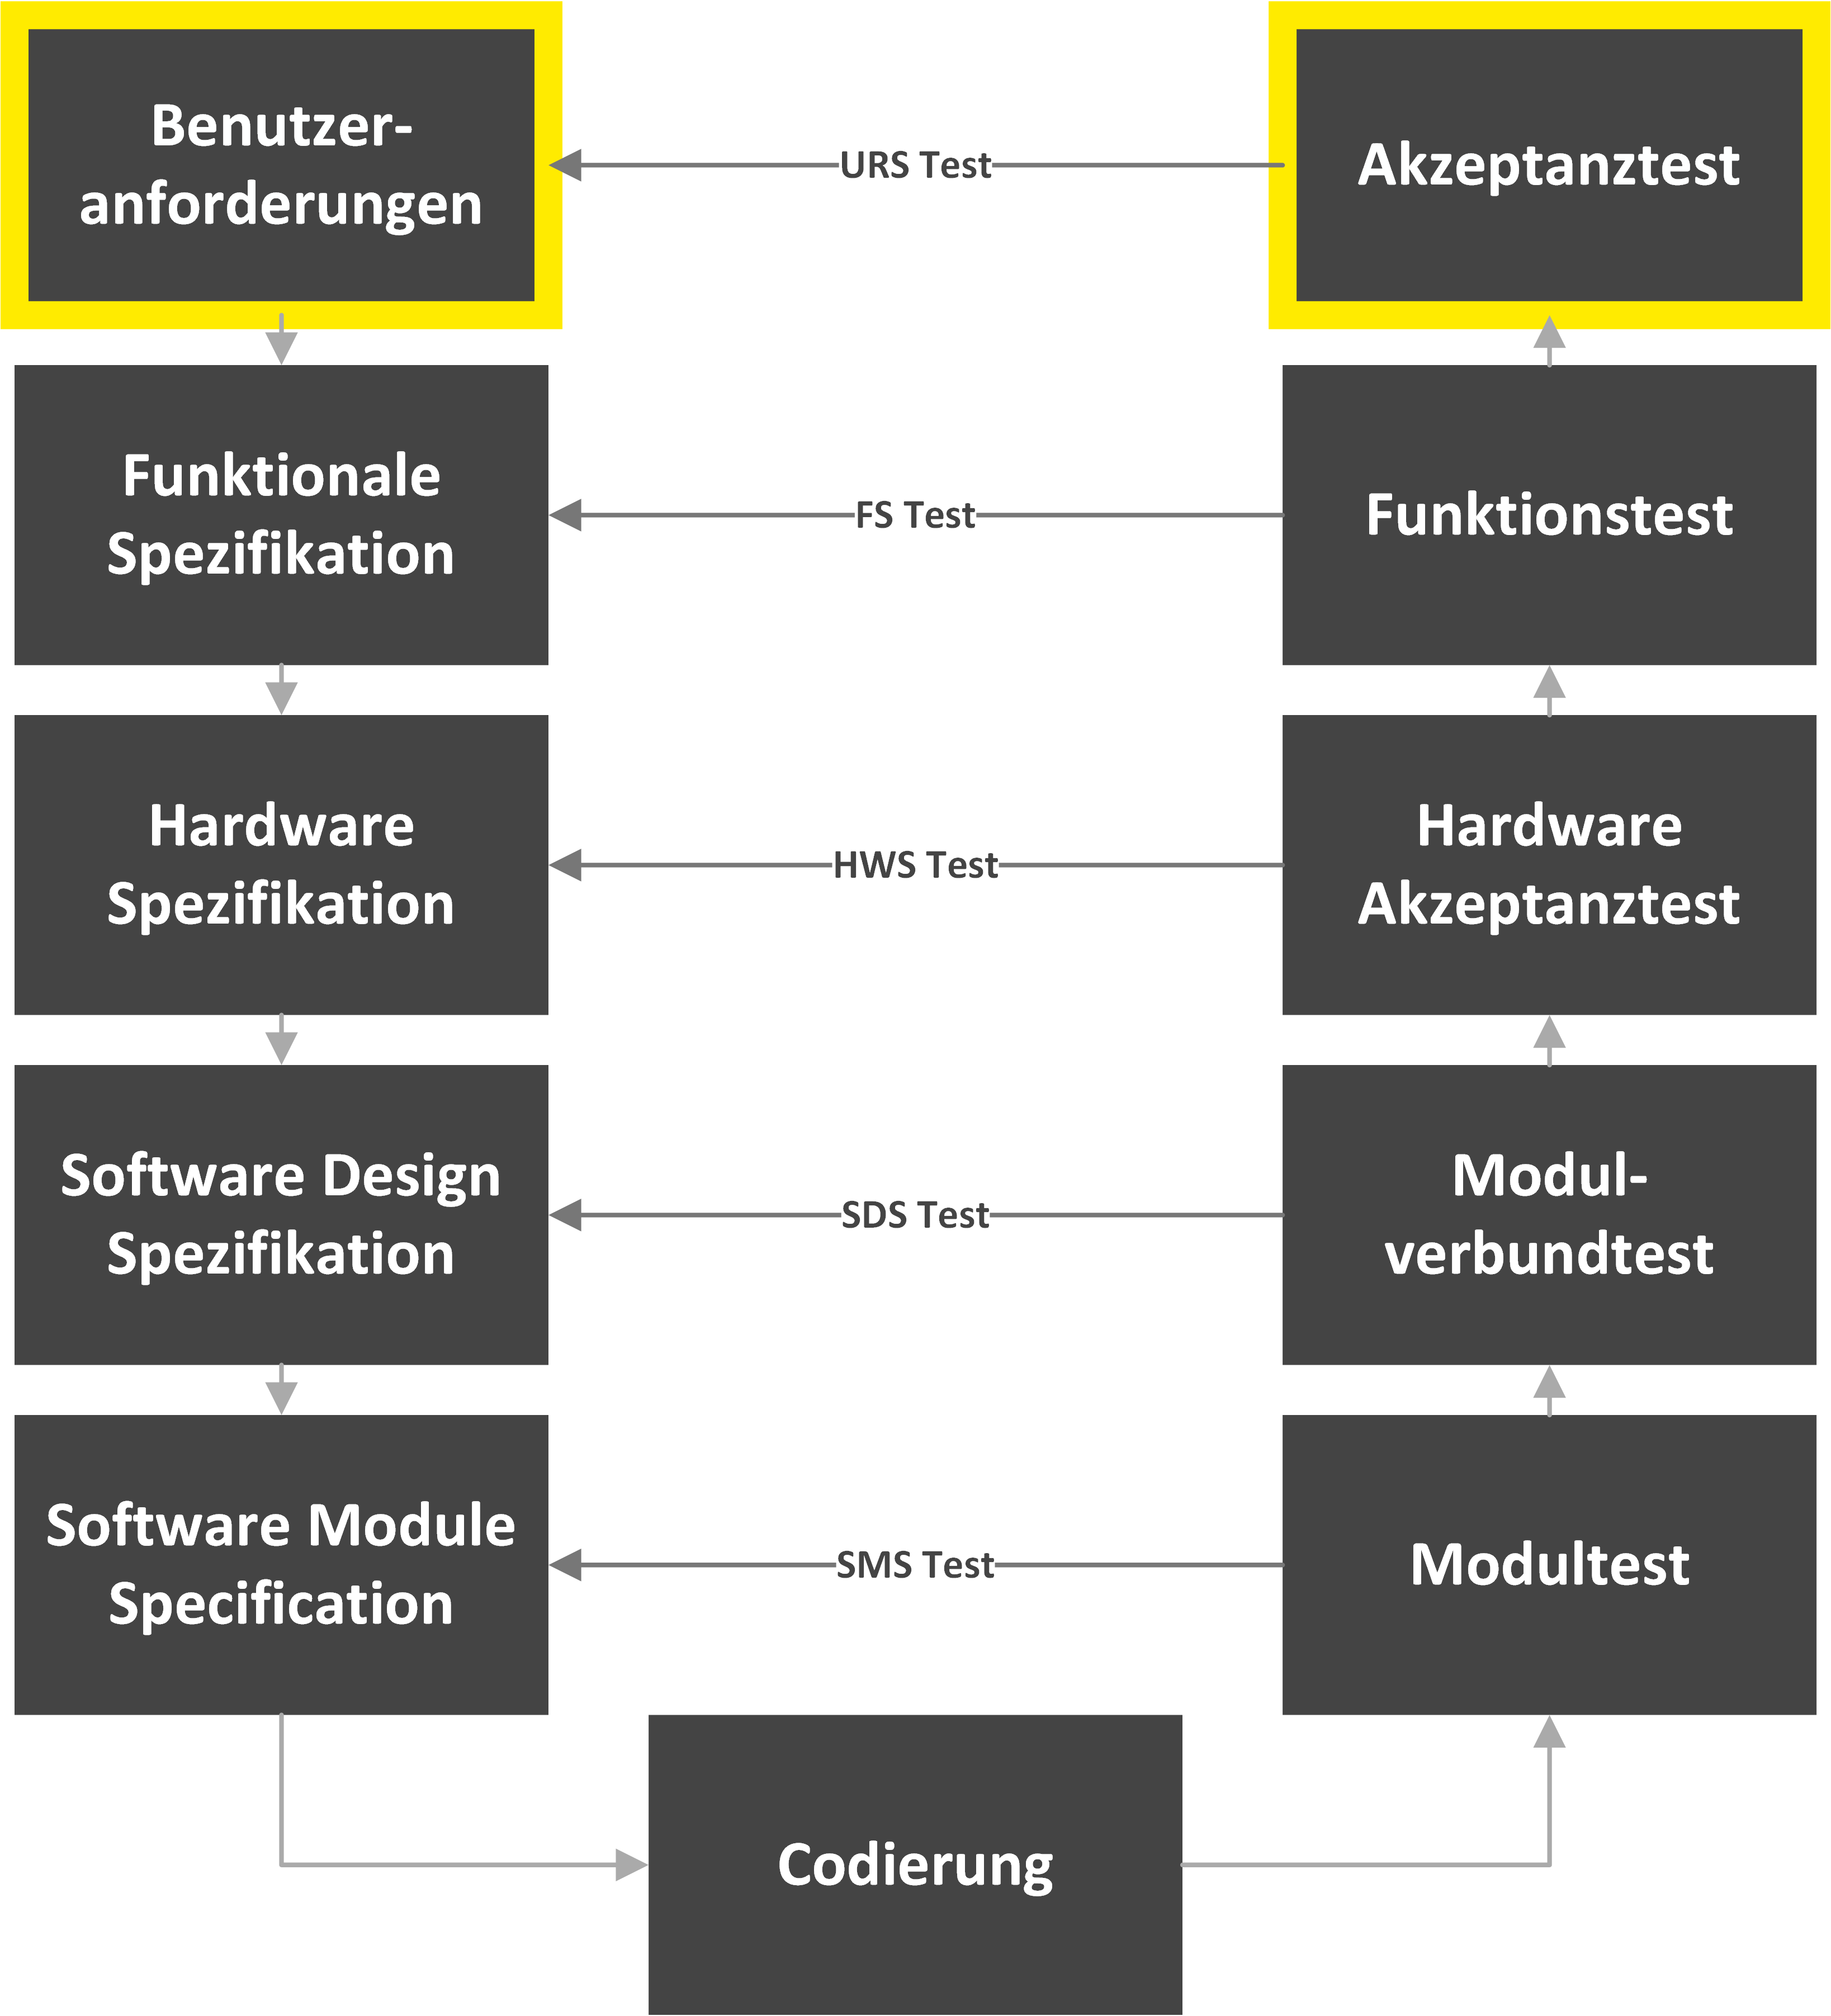
\includegraphics[width=0.4\textwidth]{V Modell 97.png}
    \caption[Vorgehen nach dem V-Modell 97]{Eigene Darstellung: Vorgehen nach dem V-Modell 97 in Anlehnung an das Skript}
    \label{abbildung_VModell97}
\end{figure}

Das Modell wurde 1991 zum ersten Mal als Protyp für ein Vorgehensmodell für Aufträge des Bundes genutzt, um dann ein Jahr später für die Projekte, die von sämtlichen deutschen Bundebehörden vergeben werden, empfohlen zu werden. Eine Bedeutung in der Privatwirtschaft fand das V-Modell im Jahr 1996 durch die Pharmaindustrie, nachdem es im selben Jahr etwas überarbeitet wurde und sowohl von der FDA als auch der Novartis gefordert beziehungsweise angewandt wurde. Das V-Modell ist mittlerweile vor allem im Wehrbereich sowie in der Pharmaindustrie anzufinden, da dort hohe Risiken auftreten und die Auftragsvergabe meist das Modell erfordert.

\begin{table}[H]
    \centering
    \begin{tabulary}{\textwidth}{|>{\centering}p{0.5\textwidth}|p{0.5\textwidth}|}
    \hline 
    \rowcolor{tableHeading} Vorteile & Nachteile \\ 
    \hline 
    Definiert erstmals Projektrollen & Der Kunde wurde als Projektrolle vergessen \\
    \hline
    Definiert notwendige Produkte \& Aktivitäten & Das Modell ist sehr umfangreich und benötigt viel Erfahrung \\
    \hline
    Kompatibilität zu \textit{ISO 12207} \& \textit{ISO 9000ff} & Das Modell ist schlecht anpassbar \\
    \hline 
    Breite Akzeptanz \& Nachfrage durch verschiedene Stellen & Unpassend für moderne Prozesse. Iterativ-inkrementelle Prozesse werden nicht unterstützt. \\
    \hline
    \end{tabulary} 
    \caption[Vor- und Nachteile des V-Modell 97]{Vor- und Nachteile des V-Modell 97}
    \label{tabelle_VModell97VorNachteile}
\end{table}

\subsubsection{V-Modell XT}
Um die bis Dato beschriebenen Probleme zu lösen, wurde im Jahre 2004 das \textbf{V-Modell XT} entworfen, welches es sich zum Ziel macht durch den einbau eines \textit{iterativen Kerns} besser für moderne Entwicklungsprozesse geeignet zu sein. Durch die Aufteilung in Vorgehensbausteine, welche eine Rolle (den Verantwortlichen) und mehrere Produkte und Aktivitäten kapseln, ist das neue Modell außerdem besser anpassbar und erweiterbar. Außerdem sollte das Modell besser skalieren und an aktuelle Normen angepasst sein.

\begin{figure}[H]
    \centering
    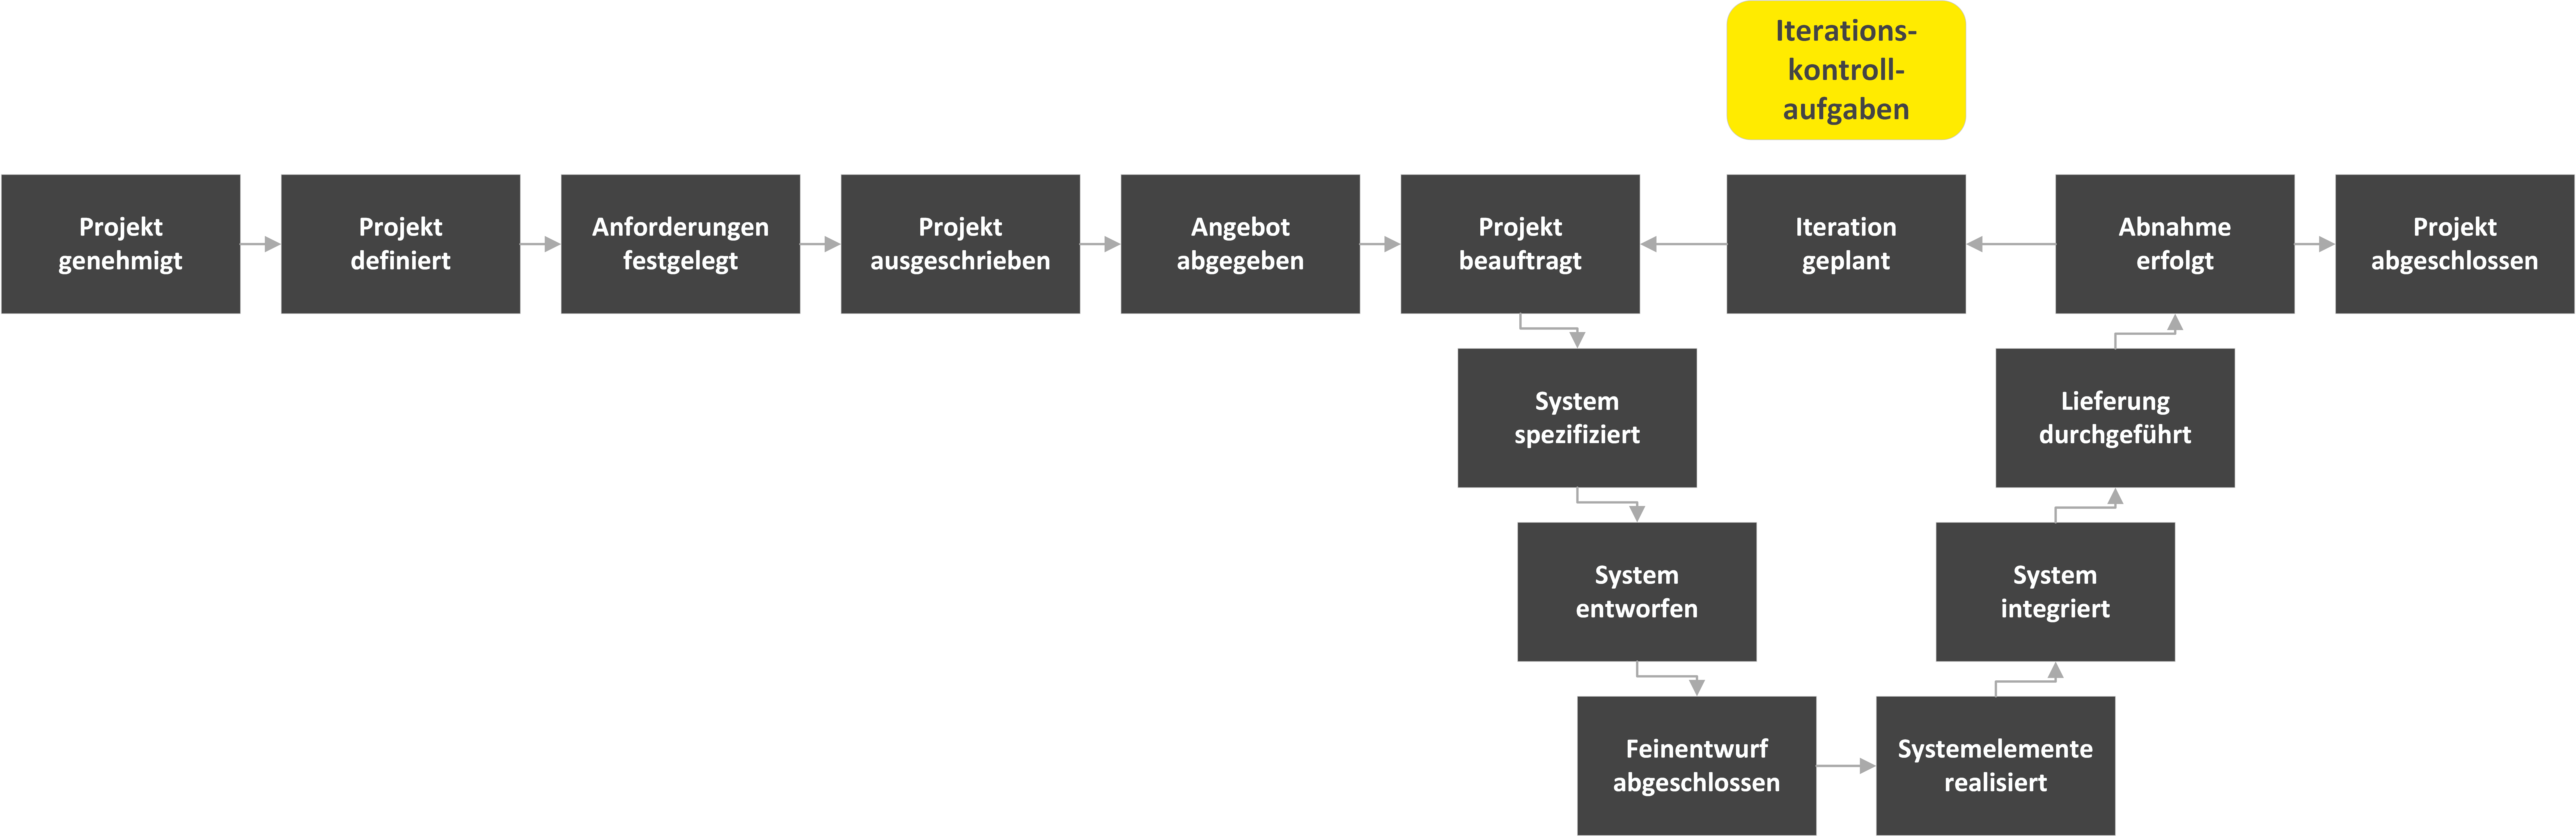
\includegraphics[width=0.4\textwidth]{V Modell XT.png}
    \caption[Vorgehen nach dem V-Modell XT]{Eigene Darstellung: Vorgehen nach dem V-Modell XT in Anlehnung an das Skript}
    \label{abbildung_VModellXT}
\end{figure}

Wie in Abbildung \ref{abbildung_VModellXT} zu sehen ist, enthällt das Modell noch immer das typische \textbf{V}, jedoch beginnt der Prozess zunächst in Phasen, welche nicht zum V gehören. Der iterative Teil ähnelt der Umsetzung von Teilprojekten mit dem \textit{V-Modell}. 

\begin{table}[H]
    \centering
    \begin{tabulary}{\textwidth}{|>{\centering}p{0.5\textwidth}|p{0.5\textwidth}|}
    \hline 
    \rowcolor{tableHeading} Vorteile & Nachteile \\ 
    \hline 
    Kompatibilität zu \textit{ISO 12207} & Noch immer sehr Umfangreich \\
    \hline 
    Technische Kompatibilität zu \textit{ISO 9000ff} & Viel Erfahrung notwendig \\
    \hline
    Ungeschmälerte Akzeptanz und Nachfrage & Qualitätsmanagement findet nur auf Projektebene statt \\
    \hline
    Erfahrung ist vorhanden &  \\ 
    \hline
    Besser Skalierbar &  \\ 
    \hline
    Tailoring ermöglicht Fokussierung auf wichtige Dokumente &  \\
    \hline
    \end{tabulary} 
    \caption[Vor- und Nachteile des V-Modell XT]{Vor- und Nachteile des V-Modell XT}
    \label{tabelle_VModellXTVorNachteile}
\end{table}

\textit{Es lässt sich zusammenfassen, dass das V-Modell jenes Modell ist, das verwendet wird, weil man es muss.} Verschiedene Stellen wie Bundesbehörden, die FDA und auch die Pharmaindustrie fordern die Umsetzung schlichtweg für ihre Projekte.